% !TeX root = Sprawozdanie.tex

\documentclass[12pt, a4paper]{article}
\usepackage{graphicx}
\usepackage[T1]{fontenc}
\usepackage[margin=0.5in,footskip=0.25in]{geometry}
\usepackage[polish]{babel}
\usepackage{hyperref}
\usepackage{amsmath}
\hypersetup{
    colorlinks=true,
    linkcolor=blue,
    filecolor=magenta,      
    urlcolor=blue,
    pdftitle={Badanie wskaźnika giełdowego MACD},
    pdfpagemode=FullScreen,
    }
\graphicspath{{./plots/}}

\title{Metody numeryczne - Badanie wskaźnika giełdowego MACD}
\author{Krzysztof Nasuta, s193328}
\date{\today}

\begin{document}
\maketitle

\section{Wstęp}

\subsection{Wskaźnik giełdowy MACD}
Celem projektu jest zaimplementowanie wskaźnika giełdowego MACD (ang. Moving Average Convergence Divergence)
oraz przeprowadzenie analizy jego skuteczności. Celem wskaźnika MACD jest wykrywanie oraz rozpoznawanie
zmian trendów na rynku finansowym. MACD składa się z 2 szeregów czasowych: linii MACD oraz linii sygnałowej.
Linia MACD uzyskiwana jest jako różnica pomiędzy 2 średnimi: długoterminową oraz krótkoterminową.
Linia sygnałowa wyliczana jest jako średnia z powstałej linii MACD. Do wyliczenia średnich często
używana jest wykładnicza średnia krocząca (ang. exponential moving average, EMA). W projekcie linię MACD uzyskano jako różnicę
pomiędzy 12-dniową wykładniczą średnią kroczącą oraz 26-dniową wykładniczą średnią kroczącą. Linia sygnałowa to
9-dniowa wykładnicza średnia krocząca z linii MACD.

Interpretacja wskaźnika MACD polega na obserwacji przecięć linii MACD oraz sygnałowej. Jeśli linia MACD przecina od dołu,
to jest to sygnał do kupna oraz zapowiedź trendu wzrostowego. Analogicznie, jeśli linia MACD przecina od góry, to jest to sygnał
do sprzedaży oraz zapowiedź trendu spadkowego.

Aby wykluczyć fałszywe sygnały, można zastosować dodatkowe filtry. W projekcie zaimplementowano filtr, który wymaga, aby linie MACD oraz sygnałowa
były w trendzie przez minimalną ilość dni, zanim zostanie wygenerowany sygnał kupna lub sprzedaży.

\subsection{Implementacja}
Do Implementacji wskaźnika MACD wykorzystano język \textit{Python} oraz narzędzie
\textit{Jupyter Notebook}, wraz z bibliotekami \textit{pandas} oraz \textit{matplotlib}.
Dane do analizy pochodzą z serwisu \href{https://stooq.pl/}{stooq.pl}.
W projekcie wykorzystano dane dotyczące 5 kursów walutowych:
\small
\begin{description}
    \setlength\itemsep{0.01em}
    \item[EUR/USD] \textbf{(Euro do Dolara Amerykańskiego)}
    \item[EUR/PLN] (Euro do Polskiego Złotego)
    \item[KRW/PLN] (Won Południowokoreański do Polskiego Złotego)
    \item[KRW/USD] (Won Południowokoreański do Dolara Amerykańskiego)
    \item[USD/PLN] (Dolar Amerykański do Polskiego Złotego)
\end{description}
\small
Projekt zajmuje się głównie analizą kursu walutowego EUR/USD. Pozostałe kursy
walutowe wykorzystano do porównania skuteczności wskaźnika MACD.
Pozwala to na analizę wskaźnika MACD na różnych rynkach walutowych.

\pagebreak






\section{Dane wejściowe}

Dane wejściowe zawierają informacje o kursach od 01.01.2019 do 31.12.2023.

\begin{figure}[ht]
    \centering
    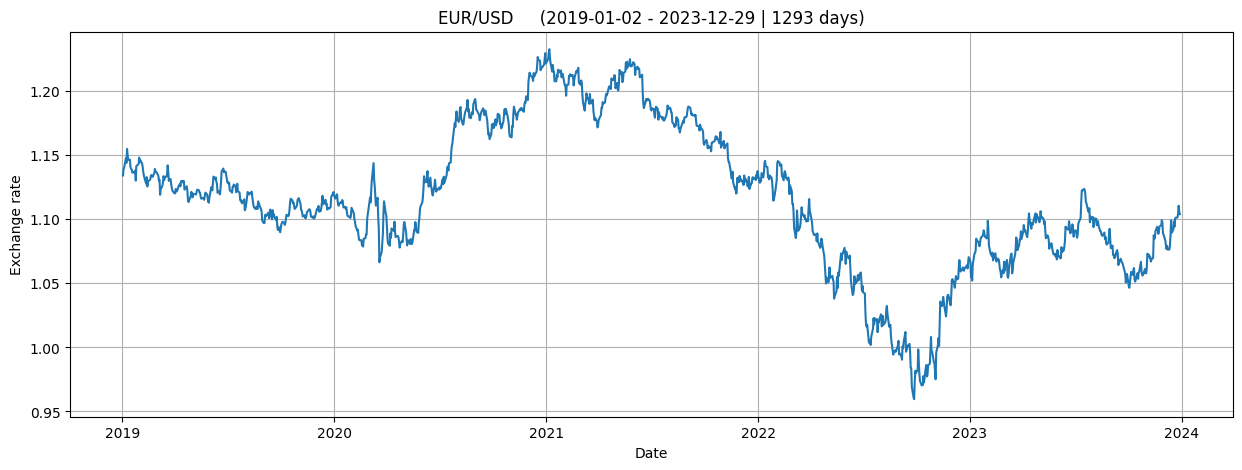
\includegraphics[width=1.0\textwidth]{eur_usd_value.png}
    \caption{Wykres kursu walutowego EUR/USD od 01.01.2019 do 31.12.2023.}
    \label{fig:eur_usd_value}
\end{figure}

\begin{center}
    Poglądowe kursy pozostałych walut:
\end{center}
\begin{figure}[ht]
    \hspace{-1cm}
    \begin{tabular}{cc}
        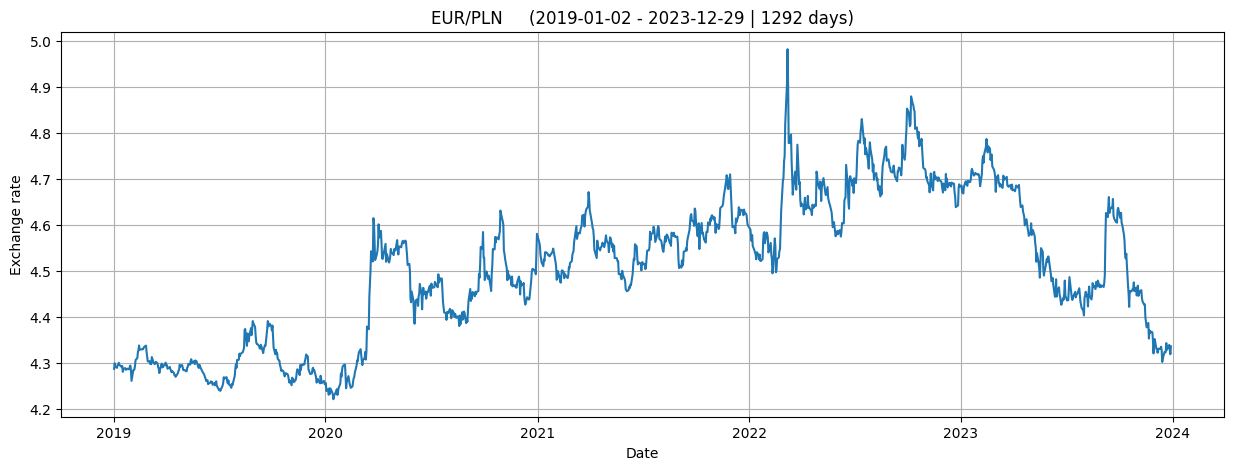
\includegraphics[width=0.5\textwidth]{eur_pln_value.png} &
        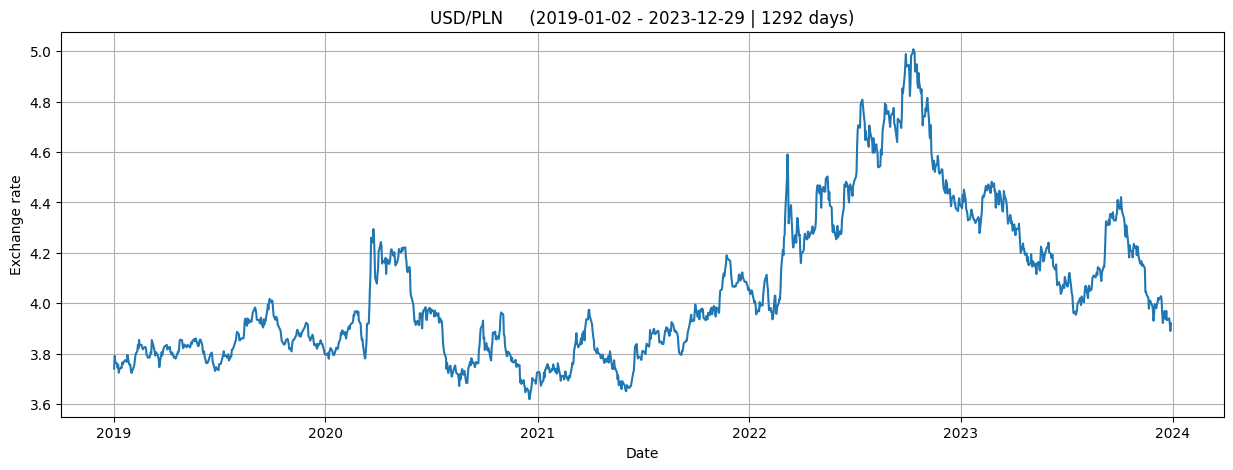
\includegraphics[width=0.5\textwidth]{usd_pln_value.png}           \\
        EUR/PLN                                                  & USD/PLN \\
        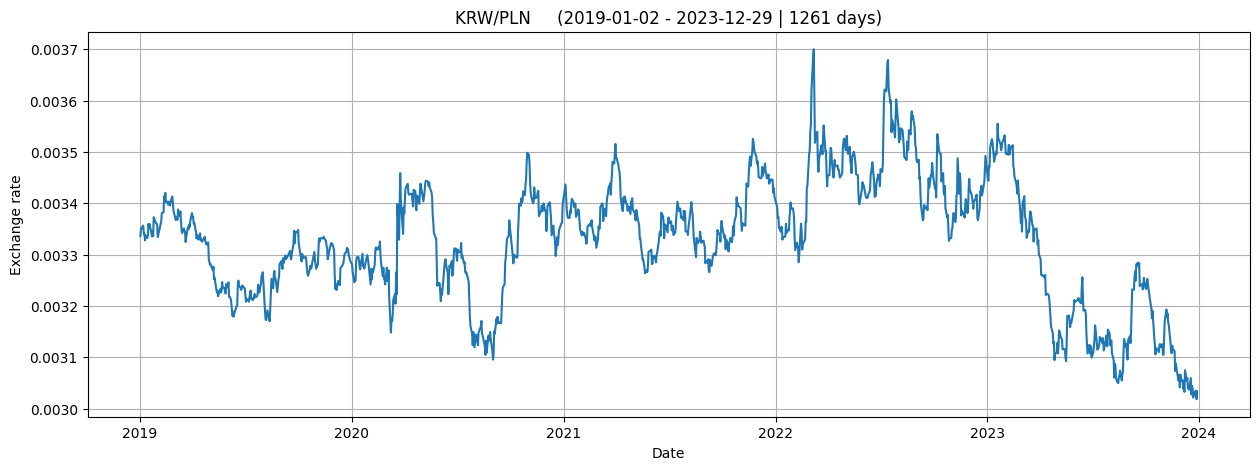
\includegraphics[width=0.5\textwidth]{krw_pln_value.png} &
        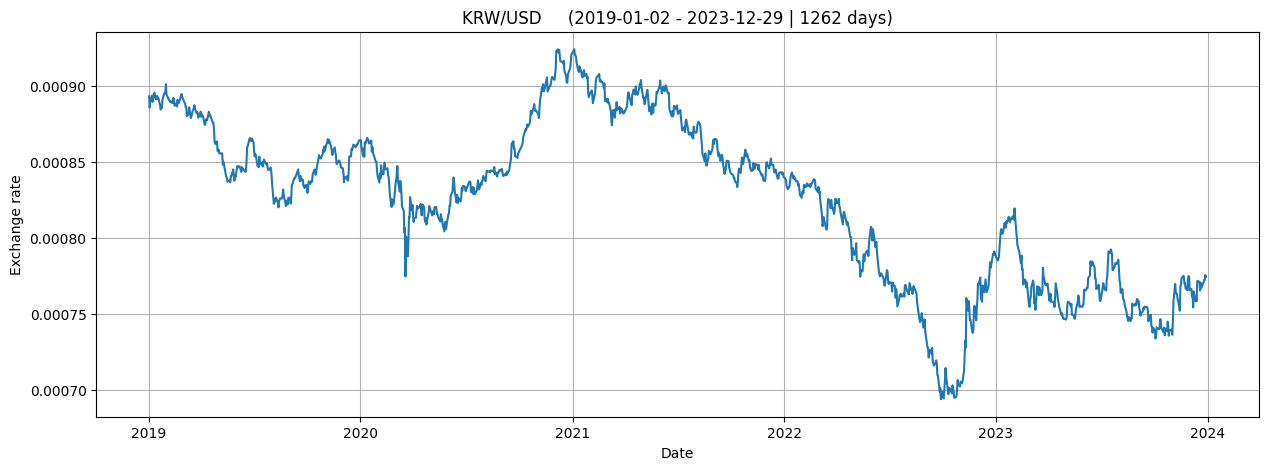
\includegraphics[width=0.5\textwidth]{krw_usd_value.png}           \\
        KRW/PLN                                                  & KRW/USD \\
    \end{tabular}
    \label{fig:other_currencies}
\end{figure}

Pełne wykresy kursów walutowych znajdują się w dodatku do sprawozdania (sekcja \ref{sec:Wykresy}).

\section{Obliczenie wskaźnika MACD dla kursu EUR/USD}

Do obliczenia wskaźnika MACD wykorzystano wzory:
\begin{equation}
    \text{MACD} = \text{EMA}_{12} - \text{EMA}_{26}
\end{equation}
\begin{equation}
    \text{SIGNAL} = \text{EMA}_{9}(\text{MACD})
\end{equation}
gdzie \textit{EMA} - wykładnicza średnia krocząca (ang. exponential moving average).

\pagebreak






Wyznaczone wskaźniki MACD oraz SIGNAL dla ostatniego 1000 notowań kursu EUR/USD
przedstawiono na poniższym wykresie:

\begin{figure}[ht]
    \centering
    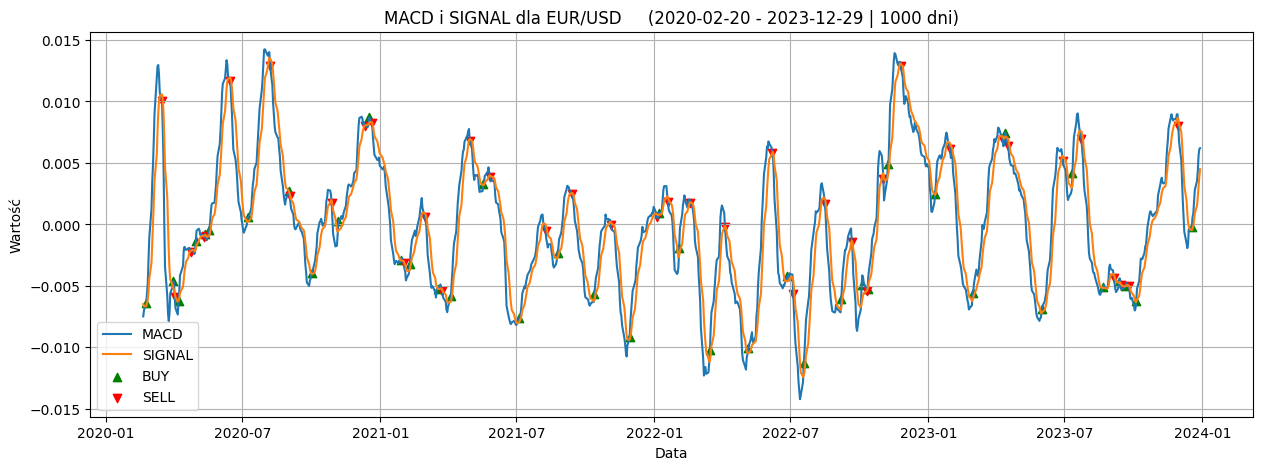
\includegraphics[width=1.0\textwidth]{eur_usd_macd_signal.png}
    \caption{Wykres wskaźnika MACD oraz SIGNAL dla kursu walutowego EUR/USD.}
    \label{fig:eur_usd_macd_signal}
\end{figure}

Wykres niebieski przedstawia wartość wskaźnika MACD, a pomarańczowy - wartość wskaźnika SIGNAL.
Na wykresie zaznaczono również punkty, w których wartości wskaźników przecinają się oraz
oznaczono je jako punkty kupna (BUY) oraz sprzedaży (SELL).
Można zauważyć, że sygnały sprzedaży generowane są zazwyczaj w momencie, gdy wartość wskaźnika MACD
jest w szczycie, a sygnały kupna w momencie, gdy wartość wskaźnika MACD jest w dołku.

Pozostałe wykresy wskaźników MACD oraz SIGNAL znajdują się w dodatku do sprawozdania (sekcja \ref{sec:Wykresy}).


\section{Analiza skuteczności wskaźnika MACD}

Z natury wskaźnika MACD wynika, że sygnały kupna oraz sprzedaży są generowane z opóźnieniem.
Nadają się one do wykrywania trendów, ale nie są odpowiednie do wykrywania szczytów oraz dołków w czasie rzeczywistym.
W związku z tym wskaźnik MACD nie jest optymalny do handlu na krótkich interwałach czasowych.
Jak można zauważyć na wykresach powyżej, niejednokrotnie sygnały kupna oraz sprzedaży
są generowane z opóźnieniem względem szczytów oraz dołków kursu walutowego. W skrajnych przypadkach
sygnały kupna oraz sprzedaży są generowane w momencie, gdy trend już się odwrócił.

Wskaźnik MACD jest także podatny na generowanie fałszywych sygnałów. Aby ograniczyć
ich liczbę, można zastosować dodatkowe filtry.

\subsection{EUR/USD}

\begin{figure}[ht]
    \centering
    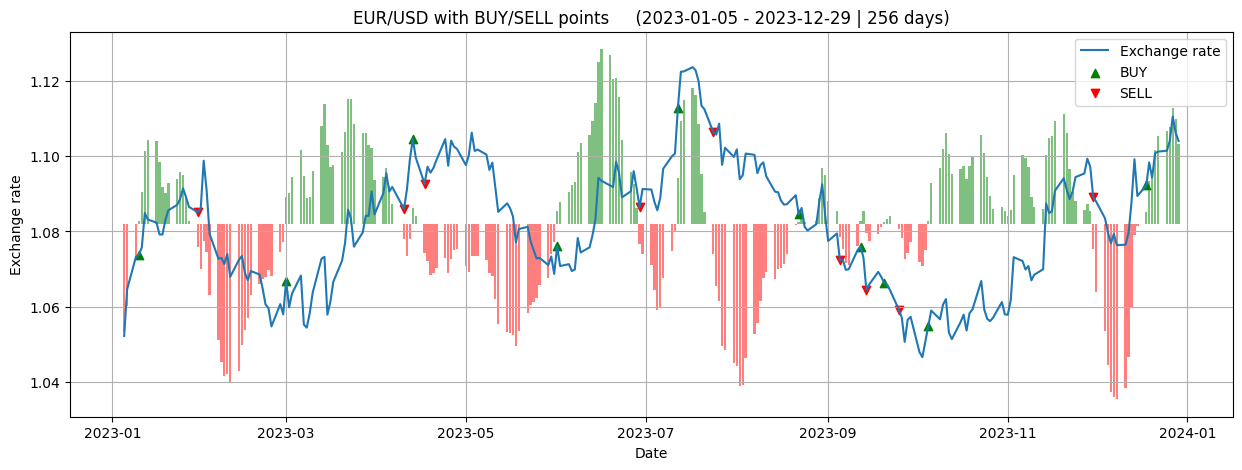
\includegraphics[width=0.8\textwidth]{eur_usd_value_buy_sell.png}
    \caption{Wykres sygnałów kupna oraz sprzedaży dla kursu walutowego EUR/USD.}
    \label{fig:eur_usd_value_buy_sell}
\end{figure}

Wykres przedstawia sygnały kupna oraz sprzedaży dla kursu walutowego EUR/USD 
nałożone na wykres kursu walutowego. Można zauważyć, że punkty przecięcia linii MACD oraz sygnałowej
zazwyczaj nie pokrywają się z szczytami oraz dołkami kursu walutowego. Zazwyczaj są one generowane
z kilkudniowym opóźnieniem. 

Wykres przedstawia również histogram wartości wskaźnika MACD. Przedstawia on różnicę
pomiędzy wartościami wskaźnika MACD oraz SIGNAL. Wykres ten potwierdza obserwacje z poprzedniego
wykresu. Jeśli pojawia się trend wzrostowy, to wartość histogramu staje się dodatnia dopiero 
po kilku dniach. Analogiczna sytuacja występuje w przypadku trendu spadkowego.



\subsection{USD/PLN}

\begin{figure}[ht]
    \centering
    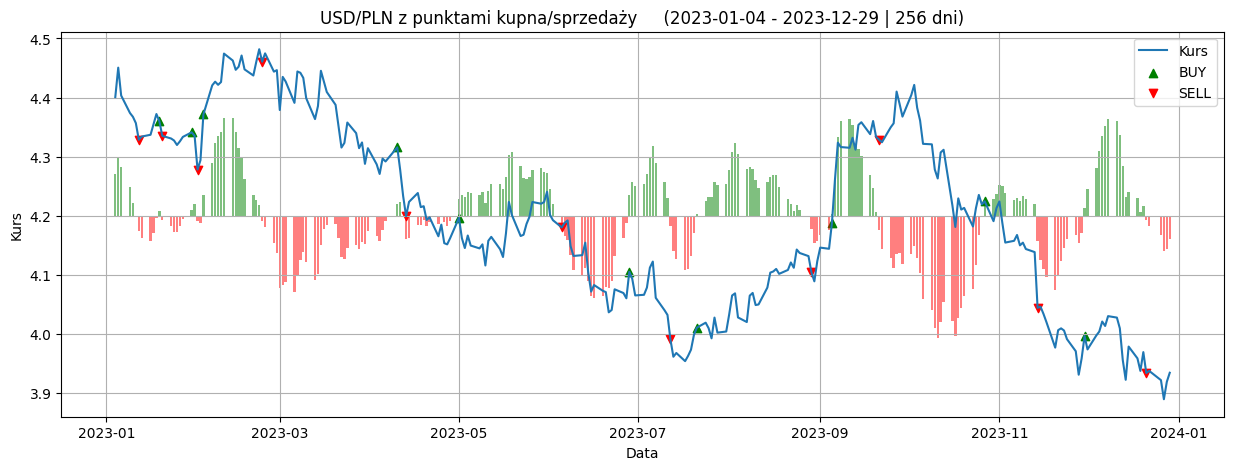
\includegraphics[width=0.8\textwidth]{usd_pln_value_buy_sell.png}
    \caption{Wykres sygnałów kupna oraz sprzedaży dla kursu walutowego USD/PLN.}
    \label{fig:usd_pln_value_buy_sell}
\end{figure}

Powyższy wykres jest analogiczny do poprzedniego. Można zauważyć, że sygnały, jak i histogram
wskaźnika MACD, są generowane z opóźnieniem względem zmian kursu walutowego. W efekcie, większość 
transakcji  kupna oraz sprzedaży przynosi małe zyski lub straty.

Wykresy dla pozostałych walut znajdują się w dodatku do sprawozdania (sekcja \ref{sec:Wykresy}).


\section{Symulacja handlu na podstawie wskaźnika MACD}

Do przeprowadzenia symulacji handlu na podstawie wskaźnika MACD, zaimplementowano
prostą strategię handlową. Strategia polega na kupnie waluty, gdy wartość wskaźnika MACD
przecina od dołu wartość wskaźnika SIGNAL oraz sprzedaży waluty, gdy wartość wskaźnika MACD
przecina od góry wartość wskaźnika SIGNAL.
Dodatkowo, zaimplementowano filtr, który wymaga, aby linie MACD oraz sygnałowa były w trendzie
przez pewną ilość dni, zanim zostanie wygenerowany sygnał kupna lub sprzedaży.

Dla każdej z 5 walut przeprowadzono symulację handlu na podstawie wskaźnika MACD. Sprawdzono również
wyniki symulacji dla różnych wartości parametru filtru, począwszy od braku filtra, aż do 5 dniowego filtra.

Za początkowy kapitał przyjęto 1000 EUR. W każdym dniu symulacji, jeśli wystąpił sygnał kupna, to cały kapitał
został zainwestowany w walutę. Analogicznie, jeśli wystąpił sygnał sprzedaży, to cała inwestycja została sprzedana.

W trakcie symulacji przeprowadzono po 54 transakcje kupna oraz sprzedaży.
Końcowy kapitał po symulacji wyniósł 1036.98 EUR, co daje zysk w wysokości 3.70\%.
Należy pamiętać, że w symulacji nie uwzględniono różnicy kursu kupna oraz sprzedaży.
W rzeczywistości zysk z transakcji byłby mniejszy.

Następnie symulację powtórzono dla różnych wartości parametru filtra.
W przypadku kursu EUR/USD, najlepsze wyniki uzyskano dla 2 dniowego filtra.
Wykorzystanie tego filtra pozwoliło na uzyskanie kapitału równego 1047.16 EUR,
co daje zysk w wysokości 4.72\%.

\pagebreak







Poniżej przedstawiono wyniki symulacji handlu dla 5 walut oraz różnych wartości parametru filtru:


\begin{center}
    \begin{table}[ht]
        \centering
        \begin{tabular}{|c||c|c|c|c|c|c|}
            \hline
            \multicolumn{7}{|c|}{\textbf{Wyniki symulacji handlu względem zastosowanego filtra}}                                           \\
            \hline
            \textbf{Waluta} & \textbf{Brak filtra} & \textbf{1 dzień} & \textbf{2 dni}  & \textbf{3 dni} & \textbf{4 dni} & \textbf{5 dni} \\
            \hline
            EUR/USD         & 3.70\%               & 2.91\%           & \textbf{4.72\%} & -0.96\%        & 1.97\%         & 0.97\%         \\
            \hline
            EUR/PLN         & \textbf{13.02\%}     & 5.68\%           & 3.53\%          & -1.59\%        & -4.07\%        & -7.66\%        \\
            \hline
            KRW/PLN         & \textbf{27.01\%}     & 26.51\%          & 22.18\%         & 6.33\%         & -1.33\%        & 3.91\%         \\
            \hline
            KRW/USD         & \textbf{4.82\%}      & 1.64\%           & -4.22\%         & -2.57\%        & -6.82\%        & -0.42\%        \\
            \hline
            USD/PLN         & 11.24\%              & \textbf{26.58\%} & 13.37\%         & 2.02\%         & -7.95\%        & -6.72\%        \\
            \hline
            \hline
            Średnia         & 11.96\%              & \textbf{12.66\%} & 7.92\%          & 0.65\%         & -3.64\%        & -1.98\%        \\
            \hline
        \end{tabular}
        \caption{Wyniki symulacji handlu dla 5 walut oraz różnych wartości parametru filtru.}
        \label{tab:results}
    \end{table}
\end{center}

Warto zauważyć, że optymalna wartość parametru filtra zależy od waluty.
Zmiana wyników symulacji w zależności od wartości parametru filtra
różni się w zależności od waluty. W średnim przypadku, najlepsze wyniki uzyskano dla 1 dniowego filtra.
Zastosowanie filtrów dłuższych niż 2 dniowe nie przyniosło pozytywnych rezultatów.

\section{Wnioski}
Dla kursu walutowego EUR/USD, wskaźnik MACD okazał się częściowo skuteczny.
Wyniki symulacji handlu na podstawie wskaźnika MACD były pozytywne, ale niezbyt znaczące.
Dla kursu EUR/USD, najlepsze wyniki uzyskano dla 2 dniowego filtra,
co pozwoliło na uzyskanie zysku w wysokości 4.72\%. Należy jednak pamiętać, że wyniki symulacji
nie uwzględniają różnicy kursu kupna oraz sprzedaży. Koszty transakcji mogą znacząco obniżyć zysk.

Z wykresu \ref{fig:eur_usd_value_buy_sell} (EUR/USD) wynika, że punkty przecięcia linii MACD oraz sygnałowej
nie zawsze pokrywają się z szczytami oraz dołkami kursu walutowego. Wynika to z natury wskaźnika MACD,
który jest opóźniony względem kursu walutowego. W efekcie większość transakcji kupna oraz sprzedaży
przyniosła małe zyski lub straty.

Bardzo dobry przykład takiej sytuacji widać na tym wykresie w okolicach 2023-07. Kurs
gwałtownie rośnie, a sygnał kupny generowany jest w momencie, kiedy kurs jest już blisko szczytu.
Następnie, po krótkim czasie kurs spada, powodując wygenerowanie sygnału sprzedaży.
W efekcie, sprzedajemy walutę w momencie, kiedy kurs jest niżej niż w momencie zakupu.

Wyniki symulacji handlu dla pozostałych walut były zróżnicowane. Dla kursu walutowego KRW/USD,
rezultat był podobny do kursu EUR/USD.

W przypadku kursu EUR/PLN, wyniki symulacji były lepsze, aczkolwiek warto zwrócić uwagę na
wykres \ref{fig:other_currencies}, na którym widać długi okres trendu wzrostowego.

Podobna sytuacja wystąpiła dla kursu USD/PLN. Warto zauważyć znaczną poprawę wyników symulacji
tego kursu po zastosowaniu 1 dniowego filtra. Może to wynikać z faktu, że kurs USD/PLN jest
bardzo zmienny, co powoduje, że częściej występują fałszywe sygnały.

Ciekawym przypadkiem jest kurs KRW/PLN, dla którego wyniki symulacji były stosunkowo dobre. Patrząc
na historię transakcji, można zauważyć, że zysk pochodzi głównie z kilku transakcji, które
dokonane zostały w drugiej połowie 2023 roku.

\section{Podsumowanie}
Wskaźnik MACD jest narzędziem, które pozwala na wykrywanie trendów na rynku finansowym.
Pozwala na ich dobrą analizę, ale nie nadaje się na generowanie sygnałów kupna oraz sprzedaży
w czasie rzeczywistym. Wynika to z faktu, że wskaźnik MACD jest znacznie opóźniony
względem kursu walutowego. Nie jest on w stanie przewidzieć, jaki kurs będzie
w przyszłości. Sygnały generowanie są za późno, co zazwyczaj powoduje
zakup bądź sprzedaż w momencie nieoptymalnym. Dodatkowo, wskaźnik MACD często
generuje fałszywe sygnały. W sytuacji ogólnej handel oparty tylko
na wskaźniku MACD nie przynosiłby zysków.

Z drugiej strony, wskaźnik MACD sprawdza się bardzo dobrze jako analityczne narzędzie
do oceny trendów na rynku. Dla długoterminowych danych pozwala na skuteczne
wykrywanie trendów wzrostowych oraz spadkowych. W połączeniu z innymi wskaźnikami
może być użyteczny do analizy rynku.


\pagebreak






\section{Wykresy}
\label{sec:Wykresy}

\subsection{EUR/USD}

\begin{figure}[ht]
    \centering
    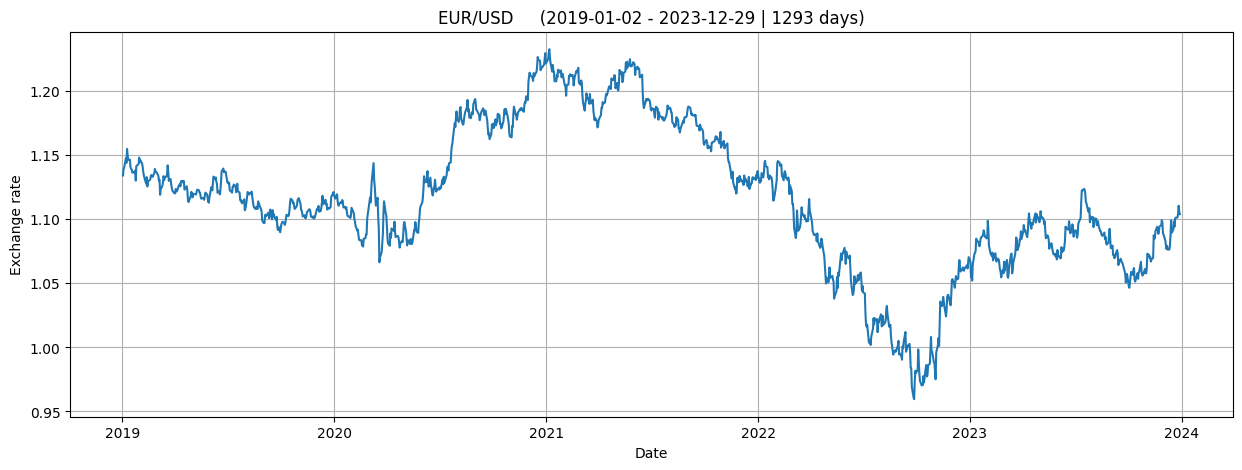
\includegraphics[width=0.77\textwidth]{eur_usd_value.png}
    \caption{Wykres kursu walutowego EUR/USD od 01.01.2019 do 31.12.2023.}
    \label{fig:all:eur_usd_value}
\end{figure}
\begin{figure}[ht]
    \centering
    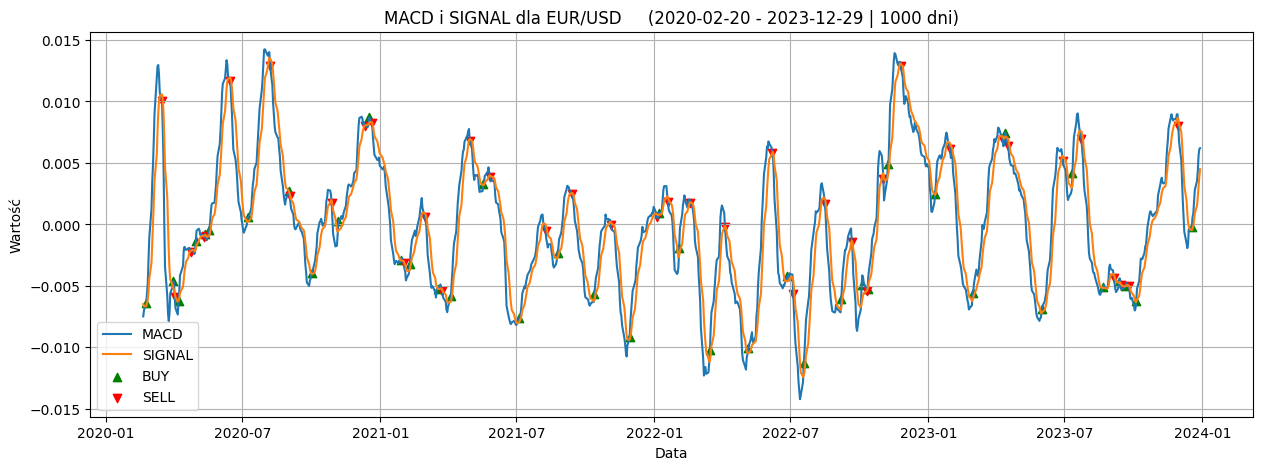
\includegraphics[width=0.77\textwidth]{eur_usd_macd_signal.png}
    \caption{Wykres wskaźnika MACD oraz SIGNAL dla kursu walutowego EUR/USD.}
    \label{fig:all:eur_usd_macd_signal}
\end{figure}
\begin{figure}[ht]
    \centering
    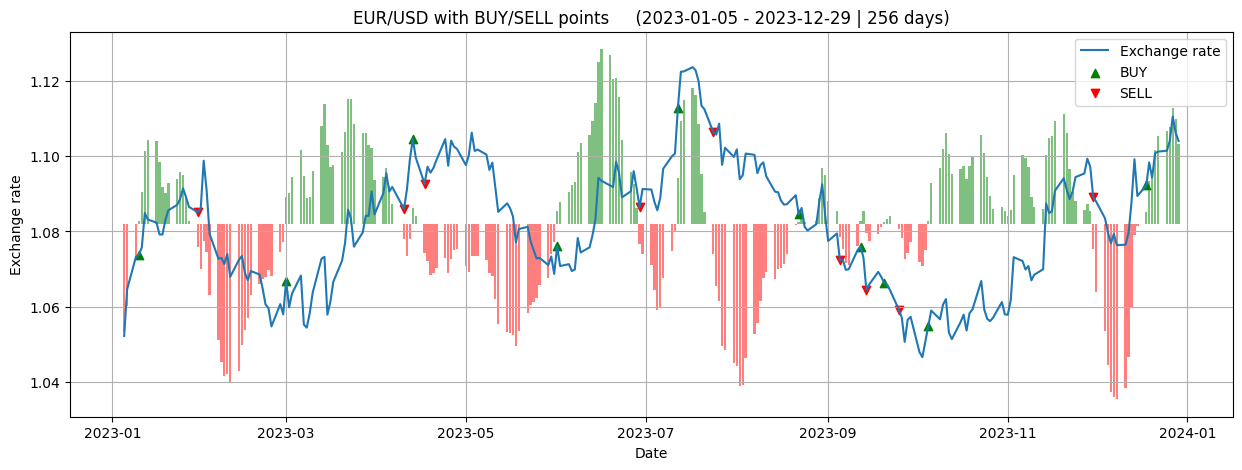
\includegraphics[width=0.77\textwidth]{eur_usd_value_buy_sell.png}
    \caption{Wykres sygnałów kupna oraz sprzedaży dla kursu walutowego EUR/USD.}
    \label{fig:all:eur_usd_value_buy_sell}
\end{figure}

\pagebreak







\subsection{EUR/PLN}

\begin{figure}[ht]
    \centering
    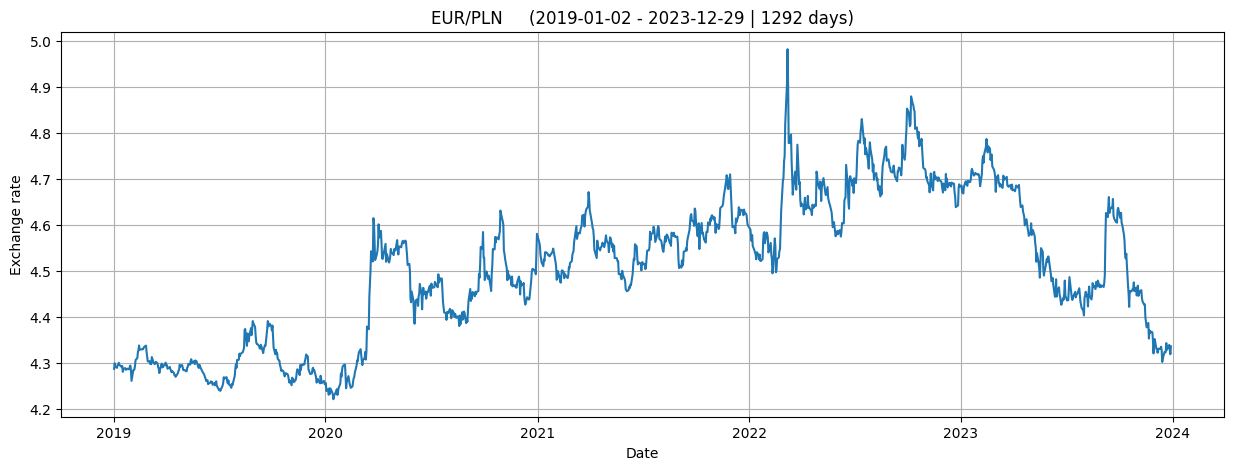
\includegraphics[width=0.77\textwidth]{eur_pln_value.png}
    \caption{Wykres kursu walutowego EUR/PLN od 01.01.2019 do 31.12.2023.}
    \label{fig:all:eur_pln_value}
\end{figure}
\begin{figure}[ht]
    \centering
    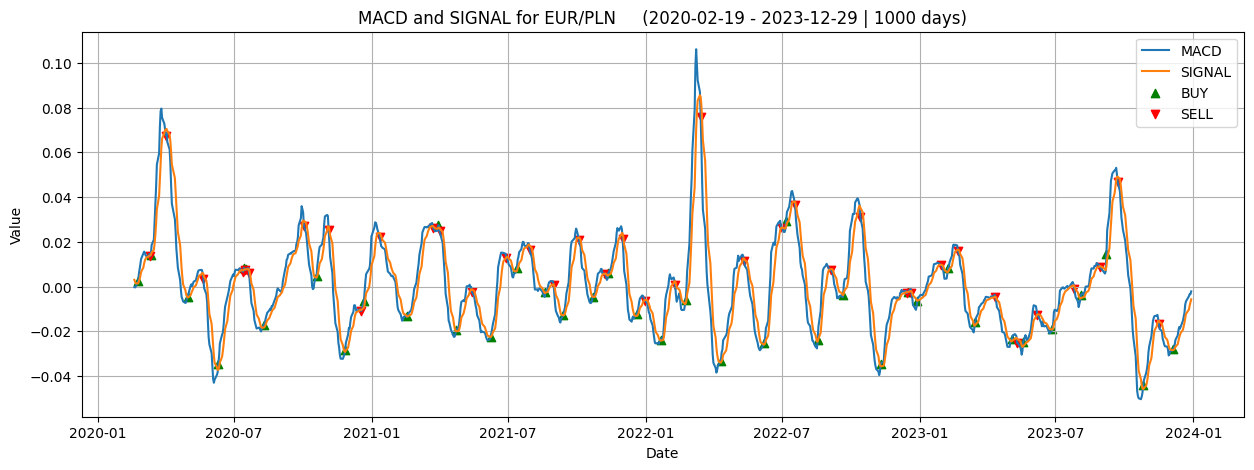
\includegraphics[width=0.77\textwidth]{eur_pln_macd_signal.png}
    \caption{Wykres wskaźnika MACD oraz SIGNAL dla kursu walutowego EUR/PLN.}
    \label{fig:all:eur_pln_macd_signal}
\end{figure}
\begin{figure}[ht]
    \centering
    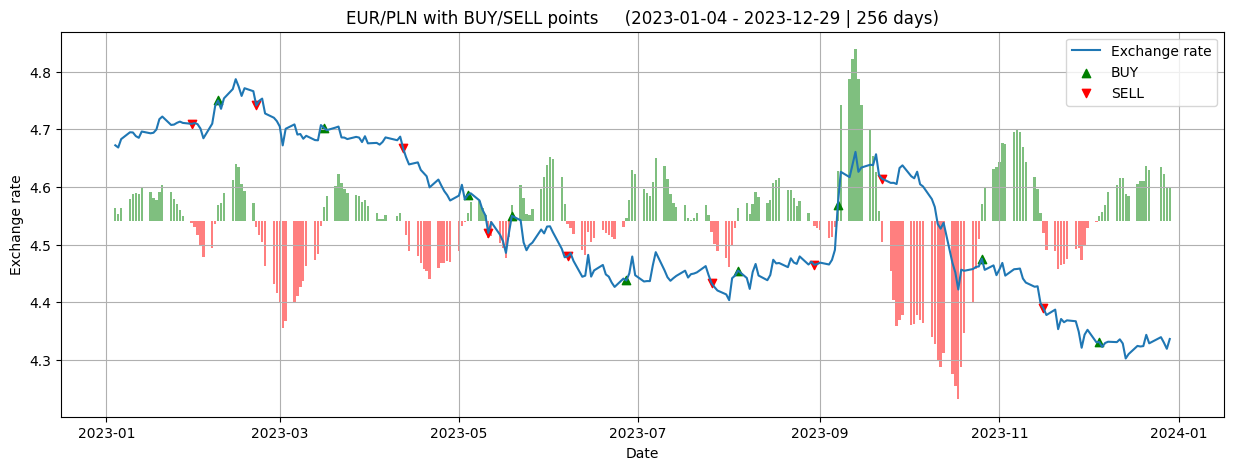
\includegraphics[width=0.77\textwidth]{eur_pln_value_buy_sell.png}
    \caption{Wykres sygnałów kupna oraz sprzedaży dla kursu walutowego EUR/PLN.}
    \label{fig:all:eur_pln_value_buy_sell}
\end{figure}

\pagebreak






\subsection{KRW/PLN}

\begin{figure}[ht]
    \centering
    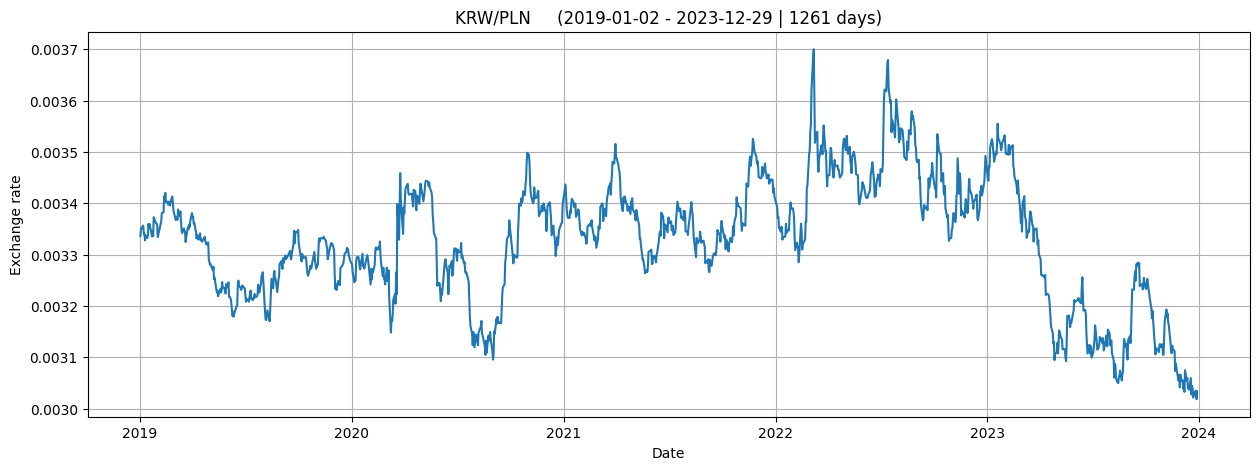
\includegraphics[width=0.77\textwidth]{krw_pln_value.png}
    \caption{Wykres kursu walutowego KRW/PLN od 01.01.2019 do 31.12.2023.}
    \label{fig:all:krw_pln_value}
\end{figure}
\begin{figure}[ht]
    \centering
    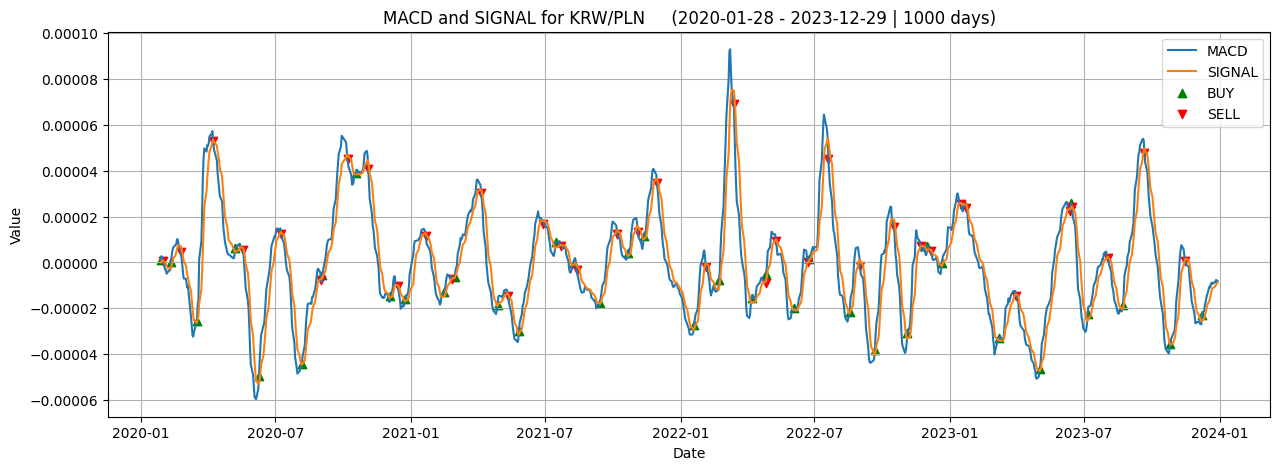
\includegraphics[width=0.77\textwidth]{krw_pln_macd_signal.png}
    \caption{Wykres wskaźnika MACD oraz SIGNAL dla kursu walutowego KRW/PLN.}
    \label{fig:all:krw_pln_macd_signal}
\end{figure}
\begin{figure}[ht]
    \centering
    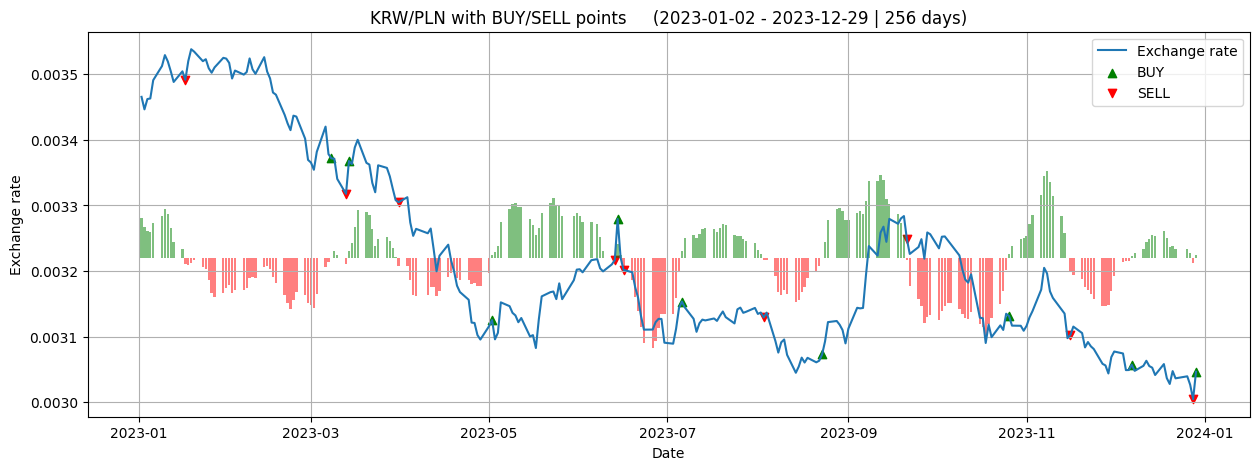
\includegraphics[width=0.77\textwidth]{krw_pln_value_buy_sell.png}
    \caption{Wykres sygnałów kupna oraz sprzedaży dla kursu walutowego KRW/PLN.}
    \label{fig:all:krw_pln_value_buy_sell}
\end{figure}

\pagebreak







\subsection{KRW/USD}

\begin{figure}[ht]
    \centering
    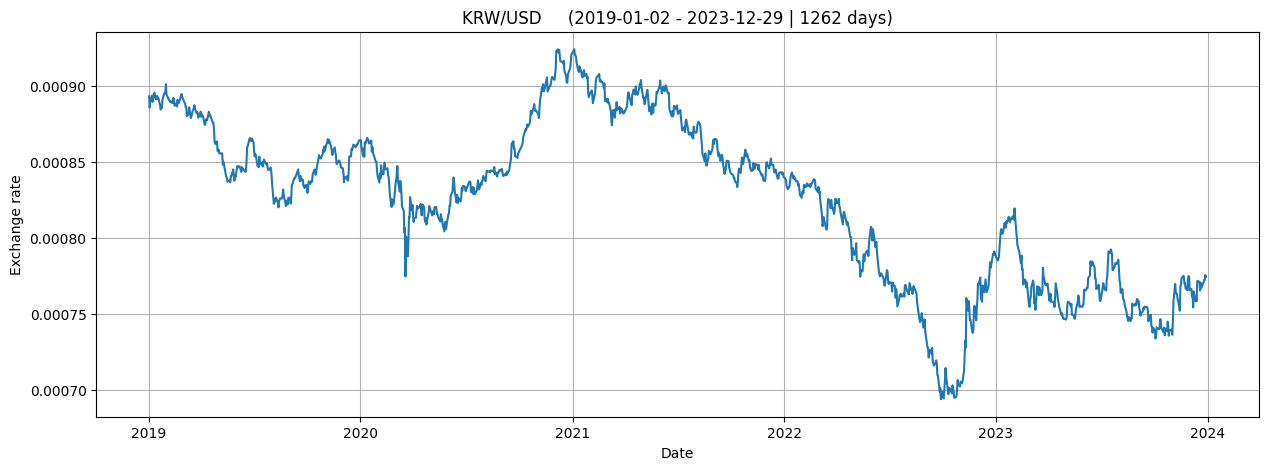
\includegraphics[width=0.77\textwidth]{krw_usd_value.png}
    \caption{Wykres kursu walutowego KRW/USD od 01.01.2019 do 31.12.2023.}
    \label{fig:all:krw_usd_value}
\end{figure}
\begin{figure}[ht]
    \centering
    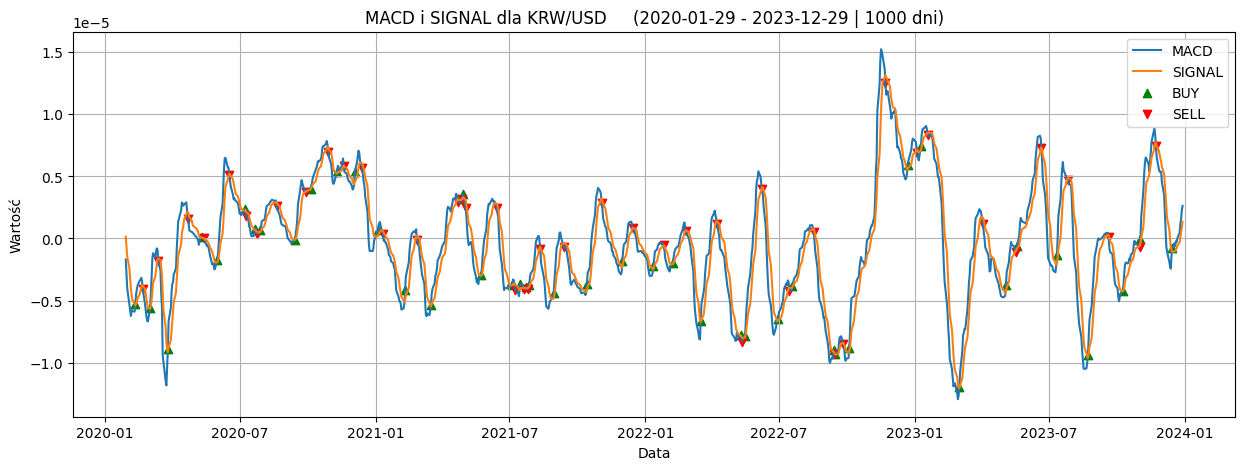
\includegraphics[width=0.77\textwidth]{krw_usd_macd_signal.png}
    \caption{Wykres wskaźnika MACD oraz SIGNAL dla kursu walutowego KRW/USD.}
    \label{fig:all:krw_usd_macd_signal}
\end{figure}
\begin{figure}[ht]
    \centering
    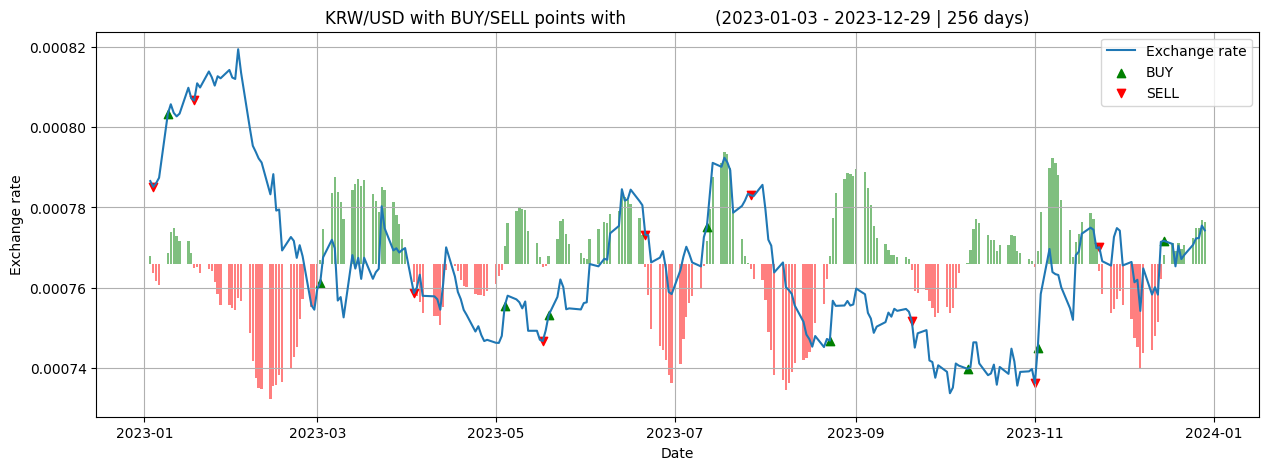
\includegraphics[width=0.77\textwidth]{krw_usd_value_buy_sell.png}
    \caption{Wykres sygnałów kupna oraz sprzedaży dla kursu walutowego KRW/USD.}
    \label{fig:all:krw_usd_value_buy_sell}
\end{figure}

\pagebreak






\subsection{USD/PLN}

\begin{figure}[ht]
    \centering
    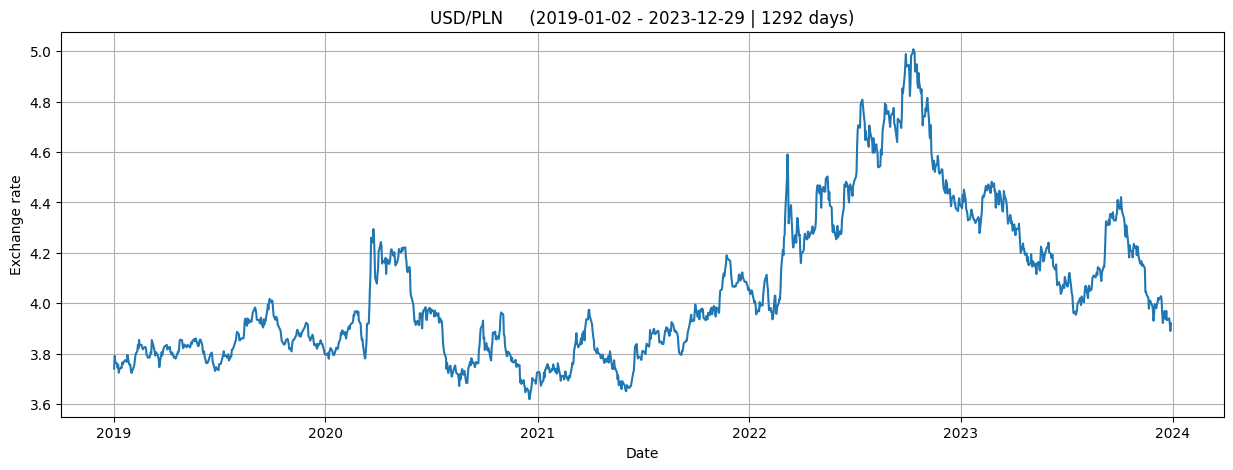
\includegraphics[width=0.77\textwidth]{usd_pln_value.png}
    \caption{Wykres kursu walutowego USD/PLN od 01.01.2019 do 31.12.2023.}
    \label{fig:all:usd_pln_value}
\end{figure}
\begin{figure}[ht]
    \centering
    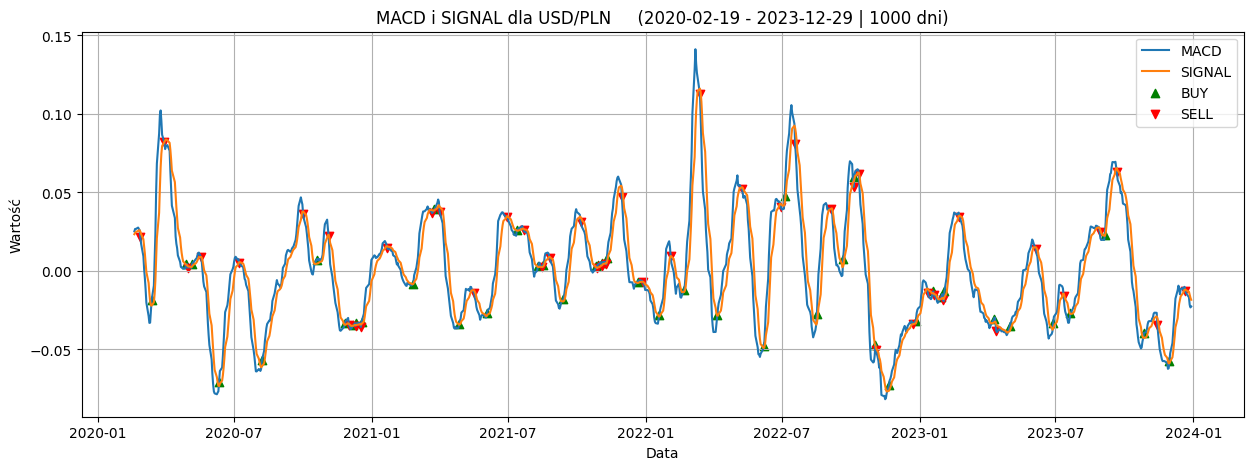
\includegraphics[width=0.77\textwidth]{usd_pln_macd_signal.png}
    \caption{Wykres wskaźnika MACD oraz SIGNAL dla kursu walutowego USD/PLN.}
    \label{fig:all:usd_pln_macd_signal}
\end{figure}
\begin{figure}[ht]
    \centering
    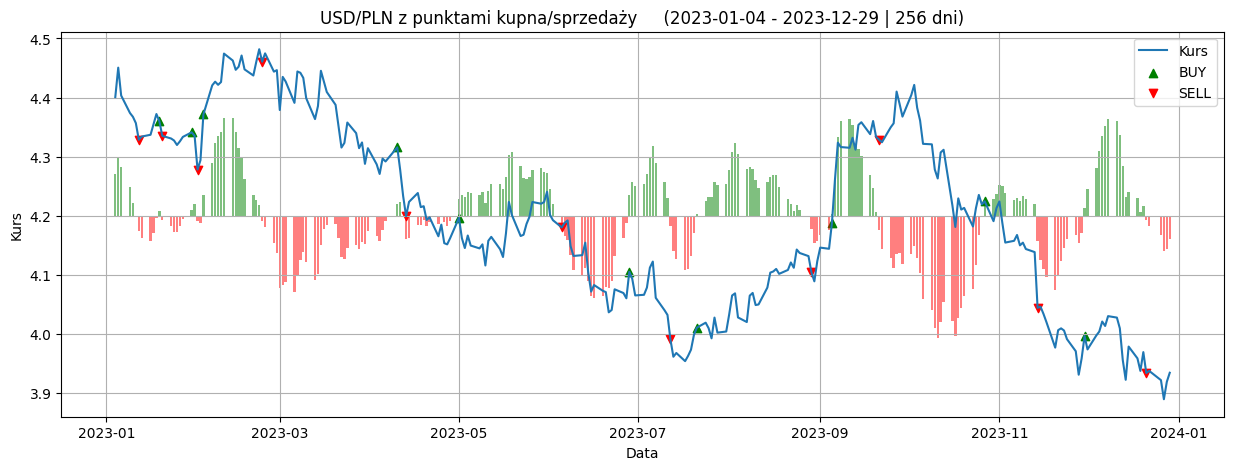
\includegraphics[width=0.77\textwidth]{usd_pln_value_buy_sell.png}
    \caption{Wykres sygnałów kupna oraz sprzedaży dla kursu walutowego USD/PLN.}
    \label{fig:all:usd_pln_value_buy_sell}
\end{figure}


\end{document}